\chapter{Tecnologías usadas}

Tomando en cuenta la información ya vertida en este documento, a continuación se explicará detalladamente la propuesta de solución.\\
En la figura \ref{fig:4-1-1} se tiene el diagrama general del sistema, se puede apreciar la comunicación entre las diferentes entidades que se usaran, que datos se mandan y reciben y por que canales transitan estos datos. A continuación se describe de manera general como es el proceso de envío y recepción de correos electrónicos ideado para este esquema.\\
\begin{enumerate}
 \item {Envío}
\begin{itemize}
\item El remitente escribe el correo electrónico y le da enviar.\\
\item El correo electrónico pasa por el complemento del cliente de correo.\\
\item El cliente genera a partir del correo una clave que usaremos para cifrar el mensaje.\\
\item Se cifra y se empaqueta el mensaje con el protocolo SMTP.\\
\item Se coloca una bandera en el mensaje.\\
\item La clave se convierte en CAPTCHA y es enviada al servidor de CAPTCHAS.\\
\item Se envía el mensaje de correo electrónico al destinatario.\\
\end{itemize}

\item{Recepción}
\begin{itemize}
\item El receptor abre un correo electrónico cifrado con el presente esquema.\\
\item El cliente lo descarga del servidor por medio del protocolo POP3 o IMAP.\\
\item Se hace una petición al servidor de CAPTCHAS para recuperar los CAPTCHAS del correo.\\
\item El usuario resuelve el CAPTCHA y se recalcula la clave de descifrado.\\
\item Se descifra el mensaje y se le muestra al usuario.\\
\end{itemize}
\end{enumerate}
\begin{figure}[h]
	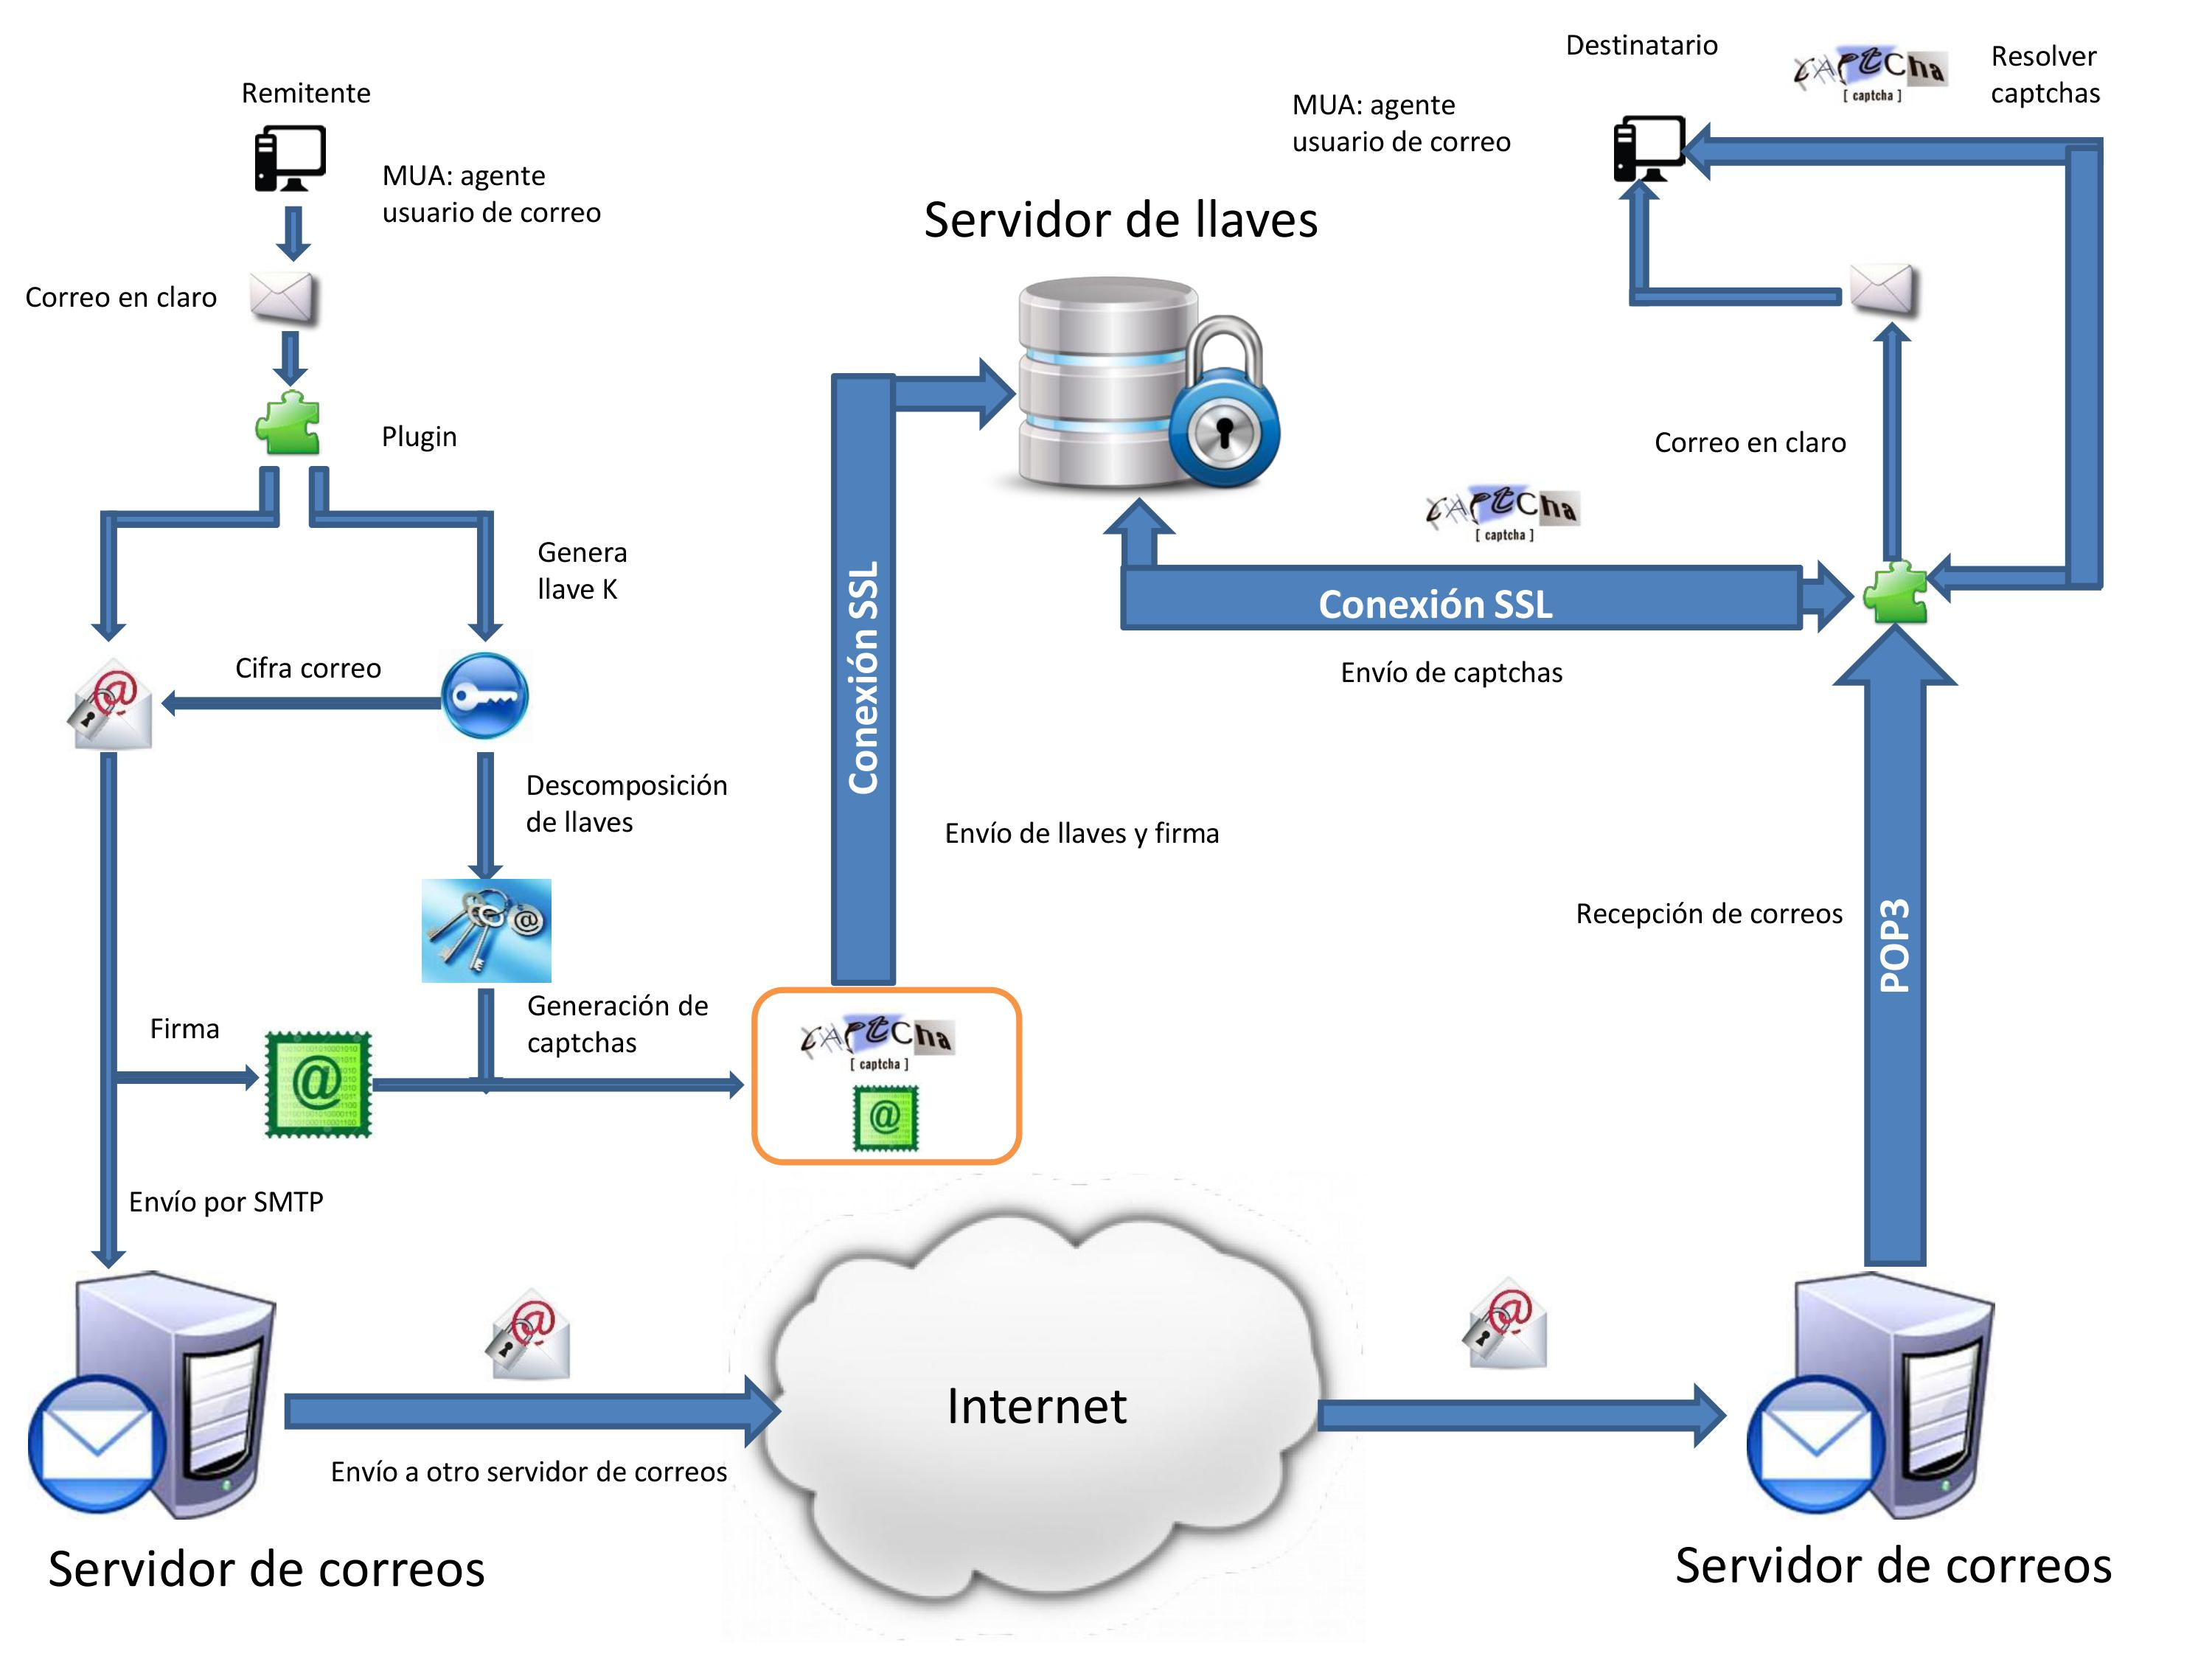
\includegraphics[width=1\linewidth, height=10cm]{./images/0001.jpg}
	\caption{Diagrama General del sistema}
	\label{fig:4-1-1}
\end{figure}
\section{Tecnologías}
Como ya se ha visto en el esquema anterior se necesita hacer uso de las herramientas adecuadas para poder desarrollar este esquema de cifrado. Las herramientas que se analizaron se describen en las siguientes secciones.\\
\subsection{Cliente de correo electrónico}
Un cliente de correo electrónico es necesario para el desarrollo de este proyecto ya que en él se instalará un complemento que cifre el mensaje, envíe los CAPTCHAS y descifre los mensajes de correo electrónico. Para ello buscamos un cliente de correo electrónico que cuente con el soporte de los protocolos POP3, SMTP y IMAP; sus licencias son de código libre; soporte la instalación de APIs externas; y tenga soporte en los sistemas operativos \textbf{\textit{Windows}}, \textbf{\textit{IOS}} y \textbf{\textit{Linux}}. Por lo tanto se investigaron los siguientes clientes de correo electrónico que se encuentra en el mercado: \\
\begin{longtable}[H]{| p{2,5cm} | p{2cm} |p{2cm}|p{1,5cm}|p{2cm}|p{3cm}|p{2cm}|}%\footnotesize
 \hline
 \textbf{Cliente de correo electrónico}&\textbf{Sistema Operativo}&\textbf{Protocolos soportados}&\textbf{Código Libre}&\textbf{Agregar funcionalidad}&\textbf{Extra}&\textbf{Gratuita o de paga}\\
 \hline
 \textbf{eM client}&Windows 7, 8 \& 10 ; IOS&POP3, SMTP, IMAP, EWS, AirSyn&NO&NO&100\% compatible con gmail y sus APIs&Ambos\\
 \hline
 \textbf{Postbox}&Windows, IOS&POP3, SMTP, IMAP&NO&SI por medio de APIs&Sincronización con Dropbox, OneDrive, Facebook y Twitter&Ambos\\
 \hline
 \textbf{Zimbra}&Windows, IOS \& Linux&POP3, SMTP, IMAP&SI&SI por medio de APIs&Una plataforma de nivel empresarial y capas se soportar sincronización con múltiples servicios&Ambos\\
 \hline
 \textbf{Opera Mail}&Windows, IOS \& Linux&POP3, SMTP, IMAP&SI&NO&La plataforma para desarrollar en Opera se actualiza cada semana&Gratuito\\
 \hline
 \textbf{Thunderbird}&Windows, IOS \& Linux&POP3, SMTP, IMAP&SI&SI por medio de APIs&Cliente de correo versátil y fácilmente escalable y una comunicad de desarrollo bastante amplia&Gratuito\\
 \hline
 \textbf{Nylas N1}&Windows, IOS \& Linux&POP3, SMTP, IMAP&SI&Si directamente compilando& &Gratuito
 
    \label{tabla:Descripcion de clientes}

\end{longtable}

\begin{itemize}
 \item El cliente de correo electrónico \textbf{\textit{eM client}} tiene una sincronización a 100\% con las cuentas de \textbf{\textit{Gmail}} y sus APIs, cuenta con una versión gratuita y una versión de paga; puede hacer migración de mensajes de correo electrónico y contactos de diversos clientes de correo electrónico y tiene una compatibilidad con muchos servidores de correo electrónico.\cite{em}\\Su desventaja es que su código es cerrado y permite agregar funcionalidades.
 \item El cliente de correo electrónico \textbf{\textit{Postbox}} esta soportada en los sistemas operativos \textbf{\textit{Windows 7}} o posteriores y \textbf{\textit{IOS}}, esta aplicación es generada por el servidor de correo electrónico \textbf{\textit{Postbox}} por lo tanto cuenta con una sincronización al 100\% con este servidor, también soporta otros servidores de correo como \textbf{\textit{Gmail}} y \textbf{\textit{Outlook}}; este cliente puede sincronizarse con \textbf{\textit{Dropbox}}, \textbf{\textit{Onedrive}} y redes sociales como \textbf{\textit{Facebook}}, \textbf{\textit{Twitter}}, entre otras. Es posible agregar más funcionalidades con la instalación de APIs.\\Una desventaja de esta aplicación es que su código es cerrado, pero gracias a que esta basado en código de \textbf{\textit{Mozilla}} puedes desarrollar APIs para agregarle tus propias funciones. \cite{box}
 \item El cliente de correo electrónico \textbf{\textit{zimbra}} es la aplicación más completa que se analizó, tiene compatibilidad con el servidor \textbf{\textit{zimbra}} pero es capaz de soportar otros servidores de correo electrónico, se encuentra en los 3 sistemas para PC, \textbf{\textit{Windows}}, \textbf{\textit{IOS}} \& \textbf{\textit{Linux}}, da la facilidad de agregarle funcionalidades por medio de la instalación de APIs y gracias a que su código es abierto se pueden programar funciones propias. Este cliente cuenta con la versión gratuita y la versión de paga. Una gran ventaja que tiene es que oferta certificaciones en el desarrollo APIs para este cliente de correo electrónico.\cite{zim}\\La única desventaja que se encontró en este cliente de correo es que la plataforma es demasiado grande y el tiempo que se necesita invertir al estudio del código es demasiado y el tiempo de desarrollo de este proyecto es muy corto.
 \item \textbf{\textit{Opera mail}} es un cliente de correo electrónico que salió al mercado recientemente y se puede instalar en los sistemas operativos \textbf{\textit{Windows}}, \textbf{\textit{IOS}} \& \textbf{\textit{Linux}}, es capaz de comunicarse con diversos servidores de correo electrónico y su código es de libre acceso.\\Su principal desventaja es que las funcionalidades que se quieran agregar no pueden ser adquiridas por medio de la instalación de complementos o APIs.\cite{opera}
 \item Por último tenemos a \textbf{\textit{Thunderbird}} que es un cliente de correo electrónico desarrollado por \textbf{\textit{Mozilla}}, este cliente es de código abierto y la instalación de APIs para agregar funcionalidad es demasiado sencilla; es un cliente de correo que puede ser instalado en los sistemas operativos \textbf{\textit{Windows}}, \textbf{\textit{IOS}} y \textbf{\textit{Linux}}.\cite{thun}
\end{itemize}
Por lo tanto el cliente de correo electrónico que se usará es \textbf{\textit{Thunderbird}}, al ser un cliente de correo electrónico casi tan completo como \textbf{\textit{zimbra}} pero con la facilidad de desarrollar APIs más rápido.\\
\subsection{Lenguajes de programación.}
Uno de los objetivos que se tienen en este proyecto es generar un complemento para un cliente de correo electrónico por lo tanto al escoger a \textbf{\textit{Thunderbird}} como cliente tenemos que programar con el lenguaje que fue desarrollado para tener la mayor compatibilidad.\\Para el desarrollo de este proyecto se utilizará\cite{thun}:
\begin{itemize}
 \item Lenguaje Python
 \item HTML 5
 \item CSS3
\end{itemize}
A pesar de ser una aplicación de escritorio este cliente de correo electrónico está construido con lenguajes web.
\subsection{Tipos de CAPTCHAS}
En el esquema de cifrado es necesario esconder la palabra que genera la clave en un CAPTCHA para ser enviado a otro usuario y descifre el mensaje, pero existen varios tipos de CAPTCHAS que se pueden utilizar\cite{cit}.\\Los CAPTCHAS se pueden clasificar de la siguiente forma:
\begin{itemize}
 \item CAPTCHAS de texto: Este tipo de CAPTCHAS genera una pregunta sencilla donde la respuesta a la pregunta es la respuesta al CAPTCHA.
 \item CAPTCHAS de imágenes: Este tipo de CAPTCHAS nos muestran en una imagen una cadena de caracteres distorsionados, esta cadena de caracteres es la repuesta del CAPCHA transformada en una imagen.
 \item CAPTCHAS de audio: Este tipo de CAPTCHAS se caracterizan por  ser un audio con ruidos de fondo, donde nos dirán la respuesta oculta.
 \item CAPTCHAS de video: Este tipo de CAPTCHAS nos muestran un video de unos cuantos segundos donde una palabra aparece alrededor de la pantalla, esta palabra es la respuesta al CAPTCHA.
 \item CAPTCHAS de acertijos: Este tipo de CPATCHAS es versatil, ya que se trata de pequeños acertijos que resolver donde la respuesta no es una palabra si no una acción o serie de acciones. Los CAPTCHAS de acertijos pueden ser armar un rompecabezas pequeño, seleccionar la imagen que no corresponde, unir figurar geométricas, etc. 
\end{itemize}
Para poder decidir qué tipo de CAPTCHAS se utilizará se consideró los siguientes puntos:
\begin{itemize}
 \item Facilidad de creación.
 \item Peso en bytes del CAPTCHA.
 \item Forma del despliegue.
 \item Tipo de respuesta.
\end{itemize}
Por lo tanto se necesita un tipo de CAPTCHA con poco peso, cuya respuesta sea una cadena de caracteres y su forma de despliegue sea fácil de implementar. \\
Considerando las necesidades anteriores las opciones son CAPTCHAS de imágenes y CAPTCHAS de texto, pero en este proyecto se utilizarán los CAPTCHAS de imágenes porque en ellos seran almacenadas las palabras claves de cifrado de los diferentes mensajes de correo electrónico y estas son cadenas de caracteres que no se les puede generar una pregunta coherente. \\
\subsection{Bases de datos para almacenar los CAPTCHAS.}
Para escoger un gestor de base de datos que controle la información de los usuarios registrados en la aplicación propuesta, la información de los  mensajes que envían entre usuarios y los CAPTCHAS asociados a los mensajes para ser descifrados se consideraron 3 características principales en un gestor base de datos relacional:\\
\begin{itemize}
 \item Rapidez en transferencias de información.
 \item Número de usuarios conectados que soporta.
 \item Facilidad de comunicación entre los lenguajes Python, HTML con los gestores de base de datos.
\end{itemize}
Los 3 gestores que se analizaron fueron SQLite, MySQL y PostGreSQL.\\
SQLite es un gestor de base de datos sumamente ligero que soporta hasta 2 terabytes de información, esta base de datos es compatible con python y lenguajes de programación web. Este gestor por su misma ligereza es posible implementarla en dispositivos móviles, pero no es recomendable cuando múltiples usuarios están haciendo peticiones al mismo tiempo ya que su rendimiento baja\cite{DB}.\\
MySQL es un gestor de base de datos que se caracteriza por su transferencia al hacer consultas de datos almacenados; es uno de los gestores libres más utilizados en aplicaciones web y cuenta con diferentes APIs para hacer la comunicación con los lenguajes Python, PHP, C++, etc. Y soporta peticiones de múltiples usuarios gracias a la implementación de hilos.\\
PostGreSQL es un gestor de base de datos que puede hacer operaciones complejas como subconsultas, transacciones y rollbacks’s. Soporta las peticiones de múltiples usuarios pero en cuanto a la velocidad de transferencia de información, comparado con MySQL, es muy lenta pero lo compensa manteniendo una velocidad casi invariable a pesar de que la base se mantenga con un número grande de registros.\cite{sql}\\
Se eligió el gestor de base de datos MySQL porque el proyecto necesita mayor rapidez en la transferencia de información más que generar filtros muy complejos para la búsqueda de información.\\
\clearpage
\chapter{An\'alisis y Dise\~no} % (fold)
\section{Diagramas de caso de uso}
Para el desarrollo de esta propuesta se muestran los siguientes diagramas del sistema.
\begin{figure}[H]
	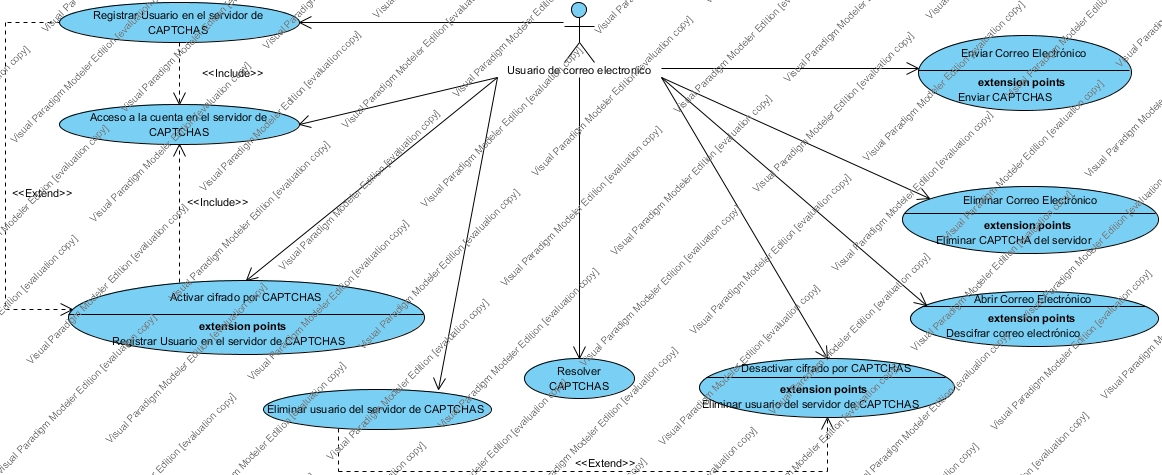
\includegraphics[width=1\linewidth, height=10cm]{./images/casodeuso1.jpg}
	\caption{Diagrama General de caso de uso}
	\label{fig:4-2-1}
\end{figure}
\subsection{Diagrama de casos de uso CU2 Registrar usuario en el servidor de CAPTCHAS}
\begin{figure}[H]
	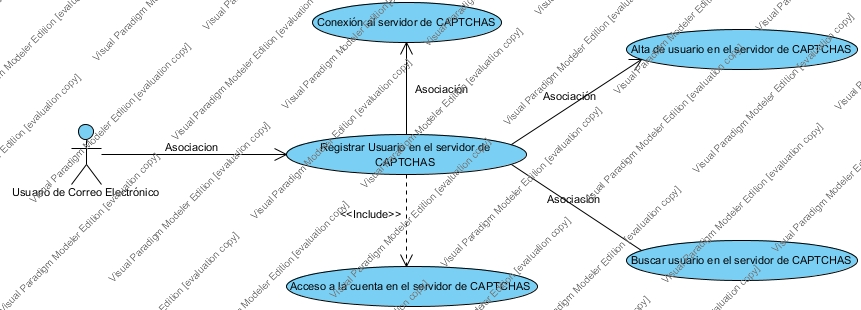
\includegraphics[width=1\linewidth, height=10cm]{./images/casodeuso2.jpg}
	\caption{Diagrama de casos de uso CU2 Registrar usuario en el servidor de CAPTCHAS}
	\label{fig:4-3-1}
\end{figure}

 \begin{longtable}[H]{| p{4,5cm} | p{0,5cm} |p{4cm}|p{5cm}|}%\footnotesize
   %\centering
   %{
     %\begin{tabular}
     \hline
     \textbf{Caso de Uso} &\multicolumn{3}{|l|}{CU2 Registrar Usuario en el servidor de CAPTCHAS}\\
     \hline
     \textbf{Actor} & \multicolumn{3}{|l|}{Actor1. Usuario de Correo Electrónico}\\
     \hline
     \textbf{Descripción} & \multicolumn{3}{|p{10cm}|}{Describe los pasos necesarios para registrar un nuevo usuario en el servidor de CAPTCHAS.}\\
     \hline
     \textbf{Pre-condiciones} & \multicolumn{3}{|l|}{Tener una cuenta de correo electrónico.}\\
     \hline
     \textbf{Post-condiciones} & \multicolumn{3}{|l|}{Activación del módulo de cifrado por CAPTCHAS.}\\
     \hline
     \textbf{Puntos de inclusión} & \multicolumn{3}{|l|}{Acceso a la cuenta en el servidor de CAPTCHAS.}\\
     \hline
     \textbf{Puntos de extensión} & \multicolumn{3}{|l|}{}\\
     \hline
     \textbf{Flujo principal} & & Actor/Sistema & Acción a realizar\\
     \hline
     & 1 & Actor & El usuario selecciona la opción registrarse en el servidor de CAPTCHAS\\
     \hline
     & 2 & Sistema & El cliente de correo contesta un formulario con la información necesaria para dar de alta en el servidor de CAPTCHAS.\\
     \hline
     & 3 & Actor & Completa el formulario y oprime el botón de registrar.\\
     \hline
     & 4 & Sistema & El sistema valida los datos proporcionados por el usuario.\\
     \hline
     & 5 & Sistema & Se conecta con el servidor y valida si el usuario ya está registrado. <FA01 - Usuario ya registrado> <FA02 - Falla en la conexión con el servidor>\\
     \hline
     & 6 & Sistema & Manda la información del usuario y lo da de alta.\\
     \hline
     & 7 & Sistema & Despliega el siguiente mensaje ``El usuario se ha dado de alta correctamente''\\
     \hline
     & & & \textbf{Fin del flujo principal}.\\
     \hline
     & \multicolumn{3}{|l|}{\textbf{FA01 - Usuario ya registrado}.}\\
     \hline
     \textbf{Flujo alternativo} & & Actor/Sistema & Acción a realizar\\
     \hline
     & 1 & Sistema & Despliega el siguiente mensaje  ``El usuario ya está registrado favor de proporcionar otra cuenta de correo electrónico''\\
     \hline
     & 2 & & El flujo continúa en el paso 3 del flujo principal.\\
     \hline
     &  & & \textbf{Fin del flujo alternativo}\\
     \hline
     
     \hline
     & \multicolumn{3}{|l|}{\textbf{FA02 - Falla en la conexión con el servidor}.}\\
     \hline
     \textbf{Flujo alternativo} & & Actor/Sistema & Acción a realizar\\
     \hline
     & 1 & Sistema & Despliega el siguiente mensaje ``La conexión con la red es nula o limitada, favor de realizar esta operación más tarde''\\
     \hline
     & 2 & & El flujo continúa en el paso 1 del flujo principal.\\
     \hline
     &  & & \textbf{Fin del flujo alternativo}\\
     %\end{tabular}
    %}
    \caption{Descripción CU2.}
    \label{tabla:CU2}
\end{longtable}


\subsection{Diagrama de casos de uso CU3 Acceso a la cuenta en el servidor de CAPTCHAS}
\begin{figure}[H]
	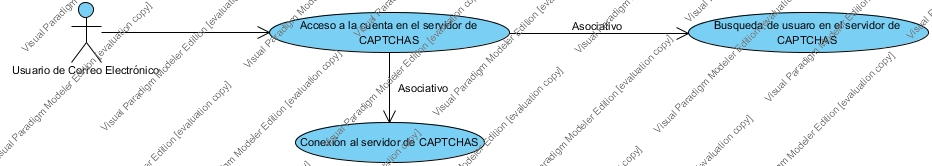
\includegraphics[width=1\linewidth, height=5cm]{./images/casodeuso3.jpg}
	\caption{Diagrama de casos de uso CU3 Acceso a la cuenta en el servidor de CAPTCHAS}
	\label{fig:4-4-1}
\end{figure}
\pagebreak

\subsection{Diagrama de casos de uso CU4 Abrir Correo Electrónico.}
\begin{figure}[H]
	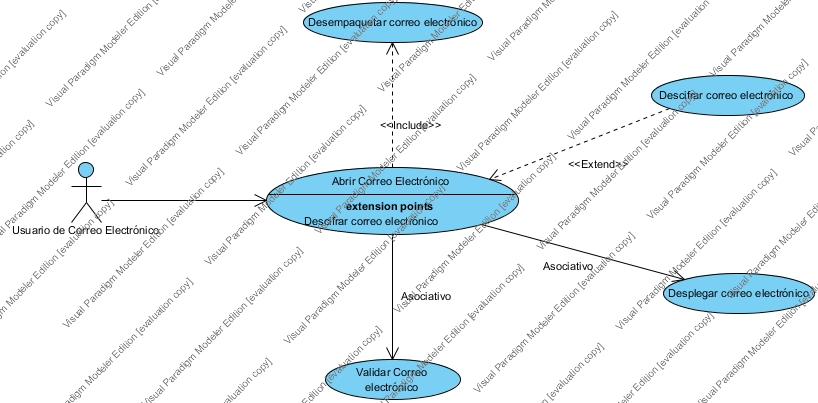
\includegraphics[width=1\linewidth, height=10cm]{./images/casodeuso4.jpg}
	\caption{Diagrama de casos de uso CU4 Abrir Correo Electrónico.}
	\label{fig:4-5-1}
\end{figure}
\begin{table}[H]
\centering
   {
     \begin{tabular}{| p{4,5cm} | p{0,5cm} |p{4cm}|p{5cm}|}
     \hline
     \textbf{Caso de Uso} &\multicolumn{3}{|l|}{CU4 Abrir correo electrónico}\\
     \hline
     \textbf{Actor} & \multicolumn{3}{|l|}{Actor 1. Usuario de correo electrónico}\\
     \hline
     \textbf{Descripción} & \multicolumn{3}{|p{10cm}|}{Describe los pasos necesarios para abrir un mensaje de correo electrónico.}\\
     \hline
     \textbf{Pre-condiciones} & \multicolumn{3}{|p{10cm}|}{1. Iniciar sesión con su servidor de correo electrónico. 2. Descargar el correo electrónico que se desea abrir.}\\
     \hline
     \textbf{Post-condiciones} & \multicolumn{3}{|l|}{Despliegue del mensaje de correo electrónico descifrado.}\\
     \hline
     \textbf{Puntos de inclusión} & \multicolumn{3}{|l|}{Desempaquetar correo electrónico}\\
     \hline
     \textbf{Puntos de extensión} & \multicolumn{3}{|l|}{Descifrar correo electrónico}\\
     \hline
     \textbf{Flujo principal} & & Actor/Sistema & Acción a realizar\\
     \hline
     & 1 & Actor & El caso de uso comienza cuando el usuario selecciona el correo que desea abrir.\\
     \hline
     & 2 & Sistema & El sistema manda a llamar a la función de desempaquetar correo electrónico.\\
     \hline
     & 3 & Sistema & Valida si el mensaje viene timbrado. <FA01 - El mensaje no viene timbrado>\\
     \hline
     & 4 & Sistema & Invoca al caso de uso <CU Descifrar correo electrónico>\\
     \hline
     & 5 & Sistema & Recibe el mensaje de correo electrónico descifrado\\
     \hline
     & 6 & Sistema & Despliega el contenido completo del mensaje al usuario\\
     \hline
     & & & \textbf{Fin del flujo principal}.\\
     \hline
     & \multicolumn{3}{|l|}{\textbf{FA01 - El mensaje no viene timbrado}.}\\
     \hline
     \textbf{Flujo alternativo} & & Actor/Sistema & Acción a realizar\\
     \hline
     & 1 & Sistema & El flujo continúa en el paso 6 del flujo principal.\\
     \hline
     &  & & \textbf{Fin del flujo alternativo}\\
     
     \end{tabular}
    }
    \caption{Descripción CU4.}
    \label{tabla:CU4}
\end{table}


\pagebreak

\subsection{Diagrama casos de uso CU5 Activar cifrado por CAPTCHAS.}
\begin{figure}[H]
	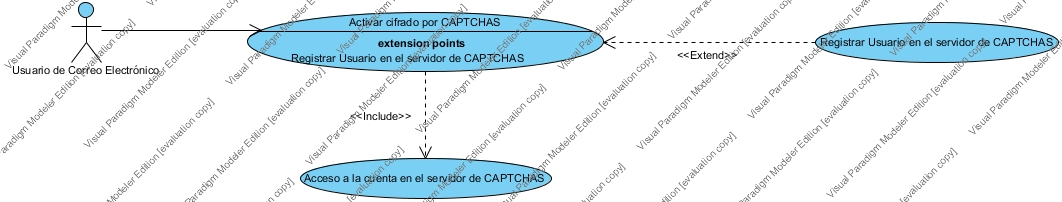
\includegraphics[width=1\linewidth, height=5cm]{./images/casodeuso5.jpg}
	\caption{Diagrama casos de uso CU5 Activar cifrado por CAPTCHAS.}
	\label{fig:4-6-1}
\end{figure}
\begin{longtable}[H]{| p{4,5cm} | p{0,5cm} |p{4cm}|p{5cm}|}
 %\centering
   %{
     %\begin{tabular}
     \hline
     \textbf{Caso de Uso} &\multicolumn{3}{|l|}{CU5 Activar cifrado por CAPTCHAS}\\
     \hline
     \textbf{Actor} & \multicolumn{3}{|l|}{Actor 1. Usuario de correo electrónico}\\
     \hline
     \textbf{Descripción} & \multicolumn{3}{|p{10cm}|}{Describe los pasos necesarios para activar el módulo de cifrado CAPTCHAS en el cliente de correo electrónico.}\\
     \hline
     \textbf{Pre-condiciones} & \multicolumn{3}{|l|}{1. Instalar el módulo de cifrado por CAPTCHAS}\\
     \hline
     \textbf{Post-condiciones} & \multicolumn{3}{|l|}{Activación del cifrado y descifrado por CAPTCHAS.}\\
     \hline
     \textbf{Puntos de inclusión} & \multicolumn{3}{|l|}{}\\
     \hline
     \textbf{Puntos de extensión} & \multicolumn{3}{|l|}{Registrar usuario del servidor de CAPTCHAS}\\
     \hline
     \textbf{Flujo principal} & & Actor/Sistema & Acción a realizar\\
     \hline
     & 1 & Actor & El caso de uso inicia cuando el actor seleccionar la opción ``Activar cifrado por CAPTCHAS''\\
     \hline
     & 2 & Sistema & El sistema verifica si la dirección de correo del usuario está registrada en el servidor de CAPTCHAS<FA01 -Usuario no registrado en el servidor>\\
     \hline
     & 3 & Sistema & Despliega una ventana con el mensaje ``Activación del módulo de cifrado por CAPTCHAS''\\
     \hline
     & & & \textbf{Fin del flujo principal}.\\
     \hline
     & \multicolumn{3}{|l|}{\textbf{FA01 -Usuario no registrado en el servidor}.}\\
     \hline
     \textbf{Flujo alternativo} & & Actor/Sistema & Acción a realizar\\
     \hline
     & 1 & Sistema & El sistema despliega una ventana con las opciones de ``Registrarse'' y ``Cancelar''. <FA02 Cancelar activación>\\
     \hline
     & 2 & Actor & Oprime el botón de ``Registrarse''\\
     \hline
     & 3 & Sistema & El sistema invoca al caso de uso <CU Registrar usuario en el servidor de CAPTCHAS>\\
     \hline
     & 4 & Sistema & El sistema obtiene una respuesta satisfactoria del registro\\
     \hline
     & 5 &  & El flujo continúa en el paso 2 del flujo principal.\\
     \hline
     &  & & \textbf{Fin del flujo alternativo}\\
     \hline
     & \multicolumn{3}{|l|}{\textbf{FA02 - Cancelar activación}.}\\
     \hline
     \textbf{Flujo alternativo} & & Actor/Sistema & Acción a realizar\\
     \hline
     & 1 & Actor & El Actor selecciona ``Cancelar''\\
     \hline
     & 2 & Sistema & Cierra la ventana de selección\\
     \hline
     & 3 &  & El flujo continúa en el paso 1 del flujo principal.\\
     \hline
     &  & & \textbf{Fin del flujo alternativo}\\
     %\end{tabular}
    %}
    \caption{Descripción CU5.}
    \label{tabla:CU5}
\end{longtable}


\pagebreak
\subsection{Diagrama de casos de uso CU6 Descifrar correo electrónico.}
\begin{figure}[H]
	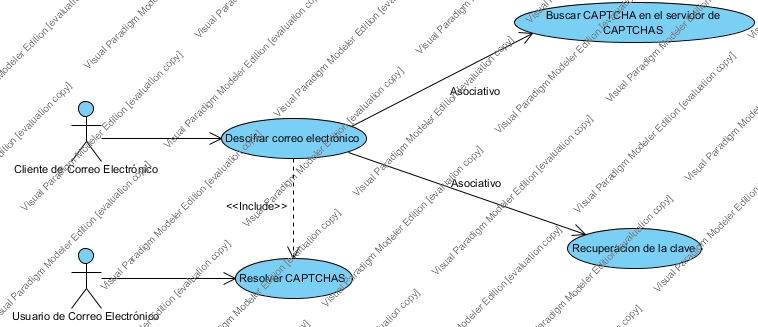
\includegraphics[width=1\linewidth, height=8cm]{./images/casodeuso6.jpg}
	\caption{Diagrama de casos de uso CU6 Descifrar correo electrónico.}
	\label{fig:4-7-1}
\end{figure}
\begin{longtable}[H]{| p{4,5cm} | p{0,5cm} |p{4cm}|p{5cm}|}
 %\centering
   %{
     %\begin{tabular}
     \hline
     \textbf{Caso de Uso} &\multicolumn{3}{|l|}{CU6 Descifrar correo electrónico.}\\
     \hline
     \textbf{Actor} & \multicolumn{3}{|l|}{Actor 1. Usuario de correo electrónico}\\
     \hline
     \textbf{Descripción} & \multicolumn{3}{|p{10cm}|}{Describe los pasos necesarios para desactivar el módulo de cifrado CAPTCHAS en el cliente de correo electrónico}\\
     \hline
     \textbf{Pre-condiciones} & \multicolumn{3}{|p{10cm}|}{1. Activar cifrado por CAPTCHAS. 2. Registrar usuario en el servidor de CAPTCHAS}\\
     \hline
     \textbf{Post-condiciones} & \multicolumn{3}{|l|}{Desactivación del cifrado y descifrado por CAPTCHAS.}\\
     \hline
     \textbf{Puntos de inclusión} & \multicolumn{3}{|l|}{}\\
     \hline
     \textbf{Puntos de extensión} & \multicolumn{3}{|l|}{Eliminar usuario del servidor de CAPTCHAS}\\
     \hline
     \textbf{Flujo principal} & & Actor/Sistema & Acción a realizar\\
     \hline
     & 1 & Actor & El caso de uso inicia cuando el actor seleccionar la opción "Desactivar cifrado por CAPTCHAS"\\
     \hline
     & 2 & Sistema & El sistema despliega la venta con las opciones de ``Desactivar cifrado'' y ``Eliminar usuario'' <FA01 - Eliminar usuario>\\
     \hline
     & 3 & Actor & Selecciona la Desactivación del cifrado por CAPTCHAS\\
     \hline
     & 4 & Sistema & El sistema desactiva el módulo de cifrado por CAPTCHA\\
     \hline
     & & & \textbf{Fin del flujo principal}.\\
     \hline
    & \multicolumn{3}{|l|}{\textbf{FA01 - Eliminar usuario}.}\\
    \hline
    \textbf{Flujo alternativo} & & Actor/Sistema & Acción a realizar\\
    \hline
    & 1 & Actor & El Actor selecciona ``Eliminar usuario''\\
    \hline
    & 2 & Sistema & El sistema despliega una ventana con las opciones de ``Aceptar'' y ``Cancelar'' para confirmar la eliminación del usuario. <FA02 - Cancelar acción eliminar usuario>\\
    \hline
     & 3 & Actor & Oprime el botón de ``Aceptar''\\
     \hline
     & 4 & Sistema & Establece la conexión con el servidor de CAPTCHAS <FA03 - Fallo en la conexión con el servidor>\\
     \hline
     & 5 & Sistema & Busca y elimina al usuario de la base de datos desplegando la confirmación del servidor.\\
     \hline
     & 6 & Actor & Oprime el botón de ``Aceptar''\\
     \hline
     & 7 & Sistema & Desactiva el módulo de cifrado por CAPTCHA\\
     \hline
     &  & & \textbf{Fin del flujo alternativo}\\
     \hline
     & \multicolumn{3}{|l|}{\textbf{FA02 - Cancelar acción eliminar usuario}.}\\
    \hline
    \textbf{Flujo alternativo} & & Actor/Sistema & Acción a realizar\\
    \hline
    & 1 & Actor & El Actor selecciona ``Cancelar''\\
    \hline
    & 2 & Sistema & Cierra la ventana de confirmación\\
    \hline
    &  & & \textbf{Fin del flujo alternativo}\\
     \hline
    & \multicolumn{3}{|l|}{\textbf{FA03 - Fallo en la conexión con el servidor}.}\\
    \hline
    \textbf{Flujo alternativo} & & Actor/Sistema & Acción a realizar\\
    \hline
    & 1 & Sistema & Despliega una ventana de alerta con el mensaje ``No se ha podido establecer la conexión con el servidor, es probable que no se tenga conexión a internet. Favor de intentarlo más tarde''\\
    \hline
    & 2 & Actor & Cierra la ventana de alerta\\
    \hline
    & 3 &  & El flujo continúa en el paso 1 del flujo principal\\
    \hline
    &  & & \textbf{Fin del flujo alternativo}\\
    % \end{tabular}
    %}
    \caption{Descripción CU6.}
    \label{tabla:CU6}
\end{longtable}


\pagebreak
\subsection{Diagrama de caos de uso CU7 Eliminar CAPTCHA del servidor.}
\begin{figure}[H]
	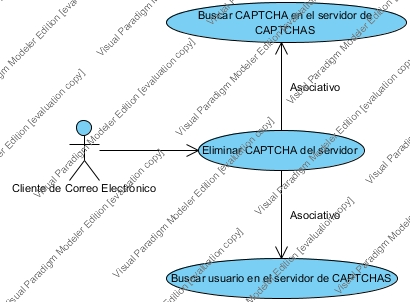
\includegraphics[width=1\linewidth, height=8cm]{./images/casodeuso7.jpg}
	\caption{Diagrama de caos de uso CU7 Eliminar CAPTCHA del servidor.}
	\label{fig:4-8-1}
\end{figure}
\begin{table}[H]
 \centering
   {
     \begin{tabular}{| p{4,5cm} | p{0,5cm} |p{4cm}|p{5cm}|}
     \hline
     \textbf{Caso de Uso} &\multicolumn{3}{|l|}{CU7 Eliminar CAPTCHA del servidor.}\\
     \hline
     \textbf{Actor} & \multicolumn{3}{|l|}{Actor 1. Cliente de correo electrónico.}\\
     \hline
     \textbf{Descripción} & \multicolumn{3}{|p{10cm}|}{Describe los pasos necesarios para eliminar los CAPTCHAS del servidor de CAPTCHAS.}\\
     \hline
     \textbf{Pre-condiciones} & \multicolumn{3}{|l|}{1. Solicitar eliminar un mensaje de correo electrónico}\\
     \hline
     \textbf{Post-condiciones} & \multicolumn{3}{|l|}{}\\
     \hline
     \textbf{Puntos de inclusión} & \multicolumn{3}{|l|}{}\\
     \hline
     \textbf{Puntos de extensión} & \multicolumn{3}{|l|}{}\\
     \hline
     \textbf{Flujo principal} & & Actor/Sistema & Acción a realizar\\
     \hline
     & 1 & Actor & Solicita eliminar CAPTCHA del servidor de CAPTCHAS\\
     \hline
     & 2 & Sistema & Busca al usuario y el CAPTCHA a eliminar en el servidor de CAPTCHAS\\
     \hline
     & 3 & Sistema & Elimina el CAPTCHA solicitado\\
     \hline
     & 4 & Sistema & Regresa la confirmación de que se eliminó el CAPTCHA.\\
     \hline
     & & & \textbf{Fin del flujo principal}.\\
          
     \end{tabular}
    }
    \caption{Descripción CU7.}
    \label{tabla:CU7}
\end{table}


\pagebreak

\subsection{Diagrama de casos de uso CU8 Eliminar correo electrónico.}
\begin{figure}[H]
	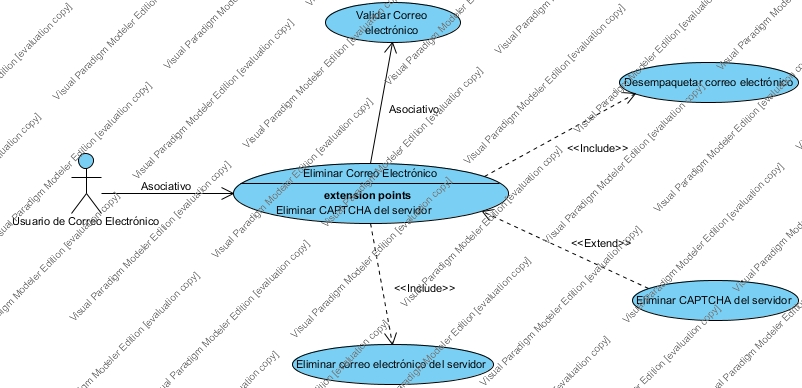
\includegraphics[width=1\linewidth, height=8cm]{./images/casodeuso8.jpg}
	\caption{Diagrama de casos de uso CU8 Eliminar correo electrónico.}
	\label{fig:4-9-1}
\end{figure}
\begin{table}[H]
 \centering
   {
     \begin{tabular}{| p{4,5cm} | p{0,5cm} |p{4cm}|p{5cm}|}
     \hline
     \textbf{Caso de Uso} &\multicolumn{3}{|l|}{CU8 Eliminar correo electrónico.}\\
     \hline
     \textbf{Actor} & \multicolumn{3}{|l|}{Actor 1. Usuario de correo electrónico.}\\
     \hline
     \textbf{Descripción} & \multicolumn{3}{|p{10cm}|}{Describe los pasos necesarios para eliminar un mensaje de correo electrónico.}\\
     \hline
     \textbf{Pre-condiciones} & \multicolumn{3}{|l|}{1. Seleccionar un mensaje de correo electrónico}\\
     \hline
     \textbf{Post-condiciones} & \multicolumn{3}{|l|}{Mensaje y CAPTCHA eliminados.}\\
     \hline
     \textbf{Puntos de inclusión} & \multicolumn{3}{|p{10cm}|}{1. Desempaquetar correo electrónico. 2. Eliminar correo electrónico del servidor}\\
     \hline
     \textbf{Puntos de extensión} & \multicolumn{3}{|l|}{Eliminar CAPTCHA del servidor de CAPTCHAS}\\
     \hline
     \textbf{Flujo principal} & & Actor/Sistema & Acción a realizar\\
     \hline
     & 1 & Actor & Selecciona un mensaje de correo electrónico a eliminar.\\
     \hline
     & 2 & Sistema & Desempaqueta el mensaje de correo electrónico\\
     \hline
     & 3 & Sistema & Valida si el mensaje esta timbrado. <FA01 - Mensaje no timbrado>\\
     \hline
     & 4 & Sistema & Invoca al caso de uso <CU Eliminar CAPTCHA del servidor>\\
     \hline
     & 5 & Sistema & Elimina el mensaje de correo electrónico y despliega el mensaje ``El correo se ha eliminado correctamente''\\
     \hline
     & & & \textbf{Fin del flujo principal}.\\
     \hline
     & \multicolumn{3}{|l|}{\textbf{FA01 - Mensaje no timbrado}.}\\
     \hline
     \textbf{Flujo alternativo} & & Actor/Sistema & Acción a realizar\\
     \hline
     & 1 & Sistema & El sistema continúa a partir del paso 5 del flujo principal.\\
     \hline
     &  & & \textbf{Fin del flujo alternativo}\\
     
     \end{tabular}
    }
    \caption{Descripción CU8.}
    \label{tabla:CU8}
\end{table}


\pagebreak
\subsection{Diagrama de casos de uso CU9 Enviar CAPTCHAS}
\begin{figure}[H]
	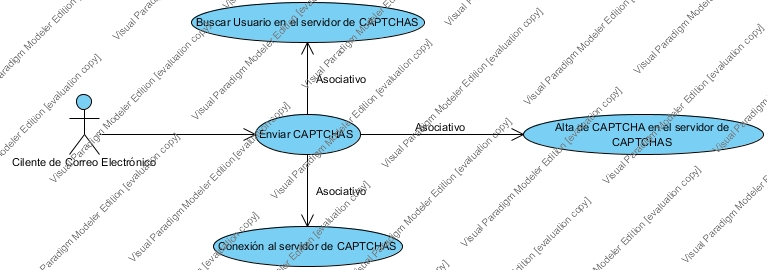
\includegraphics[width=1\linewidth, height=8cm]{./images/casodeuso9.jpg}
	\caption{Diagrama de casos de uso CU9 Enviar CAPTCHAS}
	\label{fig:4-10-1}
\end{figure}

\begin{table}[H]
 \centering
   {
     \begin{tabular}{| p{4,5cm} | p{0,5cm} |p{4cm}|p{5cm}|}
     \hline
     \textbf{Caso de Uso} &\multicolumn{3}{|l|}{CU9 Enviar CAPTCHAS}\\
     \hline
     \textbf{Actor} & \multicolumn{3}{|l|}{Actor 1. Cliente de correo electrónico.}\\
     \hline
     \textbf{Descripción} & \multicolumn{3}{|p{10cm}|}{Describe los pasos necesarios para enviar el CAPTCHA el servidor de CAPTCHAS}\\
     \hline
     \textbf{Pre-condiciones} & \multicolumn{3}{|l|}{1. Solicitar el envió de un nuevo mensaje de correo electrónico.}\\
     \hline
     \textbf{Post-condiciones} & \multicolumn{3}{|l|}{Envío del CAPTCHA al servidor de CAPTCHAS}\\
     \hline
     \textbf{Puntos de inclusión} & \multicolumn{3}{|l|}{}\\
     \hline
     \textbf{Puntos de extensión} & \multicolumn{3}{|l|}{}\\
     \hline
     \textbf{Flujo principal} & & Actor/Sistema & Acción a realizar\\
     \hline
     & 1 & Actor & Solicita el envío de CAPTCHA al servidor\\
     \hline
     & 2 & Sistema & Abre la conexión y busca al usuario en el servidor de CAPTCHAS\\
     \hline
     & 3 & Sistema & Da de alta el CAPTCHA en el servidor asociándolo con el usuario.\\
     \hline
     & 4 & Sistema & Regresa la confirmación de que se dio de alta el CAPTCHA\\
     \hline
     & & & \textbf{Fin del flujo principal}.\\
         
     \end{tabular}
    }
    \caption{Descripción CU9.}
    \label{tabla:CU9}
\end{table}


\pagebreak
\subsection{Diagrama de casos de uso CU10 Enviar correo electrónico.}
\begin{figure}[H]
	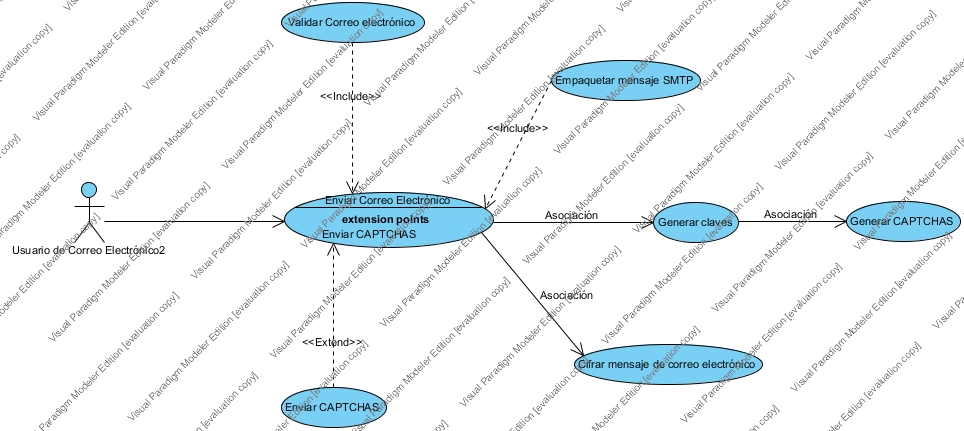
\includegraphics[width=1\linewidth, height=8cm]{./images/casodeuso10.jpg}
	\caption{Diagrama de casos de uso CU10 Enviar correo electrónico.}
	\label{fig:4-11-1}
\end{figure}
\begin{table}[H]
 \centering
   {
     \begin{tabular}{| p{4,5cm} | p{0,5cm} |p{4cm}|p{5cm}|}
     \hline
     \textbf{Caso de Uso} &\multicolumn{3}{|l|}{CU10 Enviar correo electrónico.}\\
     \hline
     \textbf{Actor} & \multicolumn{3}{|l|}{Actor 1. Usuario de correo electrónico.}\\
     \hline
     \textbf{Descripción} & \multicolumn{3}{|p{10cm}|}{Describe los pasos necesarios para enviar un mensaje de correo electrónico cifrado a otro usuario de correo electrónico.}\\
     \hline
     \textbf{Pre-condiciones} & \multicolumn{3}{|p{10cm}|}{1. El usuario tiene que redactar un mensaje de correo electrónico que contenga la dirección del destinatario.}\\
     \hline
     \textbf{Post-condiciones} & \multicolumn{3}{|p{10cm}|}{Envió de un mensaje cifrado al servidor de correo electrónico y el registro del CAPTCHA en el servidor de CAPTCHAS.}\\
     \hline
     \textbf{Puntos de inclusión} & \multicolumn{3}{|p{10cm}|}{1. Validar correo electrónico. 2. Empaquetar mensaje de correo electrónico SMTP.}\\
     \hline
     \textbf{Puntos de extensión} & \multicolumn{3}{|l|}{Enviar CAPTCHA}\\
     \hline
     \textbf{Flujo principal} & & Actor/Sistema & Acción a realizar\\
     \hline
     & 1 & Actor & Oprime el botón ``Enviar''\\
     \hline
     & 2 & Sistema & Valida que el mensaje de correo electrónico contenga los datos mínimos.<FA01 - Campos no completados>\\
     \hline
     & 3 & Sistema & Genera una llave de cifrado\\
     \hline
     & 4 & Sistema & Con una palabra aleatoria se genera el CAPTCHA y cifra el mensaje de correo electrónico.\\
     \hline
     & 5 & Sistema & Toma el mensaje cifrado y es empaquetado para enviarse al servidor de correo electrónico\\
     \hline
     & 6 & Sistema & Toma el CAPTCHA  y se envía al caso de uso <CU Enviar CAPTCHA>\\
     \hline
     & 7 & Sistema & Despliega el mensaje de ``envío satisfactorio''\\
     \hline
     & & & \textbf{Fin del flujo principal}.\\
     \hline
     & \multicolumn{3}{|l|}{\textbf{FA01 - Campos no completados}.}\\
     \hline
     \textbf{Flujo alternativo} & & Actor/Sistema & Acción a realizar\\
     \hline
     & 1 & Sistema & Notifica al usuario cuales campos han sido mal proporcionados, para poder enviar el mensaje correctamente\\
     \hline
     & 2 & Actor & Modifica los campos solicitados\\
     \hline
     & 3 &  & El flujo continúa en el paso 1 del flujo principal\\
     \hline
     &  & & \textbf{Fin del flujo alternativo}\\
     
     \end{tabular}
    }
    \caption{Descripción CU10.}
    \label{tabla:CU10}
\end{table}



\pagebreak
\section{Diagramas a bloques}
A continuación se presentan los diagramas a bloques, en donde se muestra cuál es la secuencia de procesos a realizar. Esto servirá para comprender cómo se comunican los diferentes módulos de manera interna, y cómo hacen los procesos.


\begin{figure}[H]
	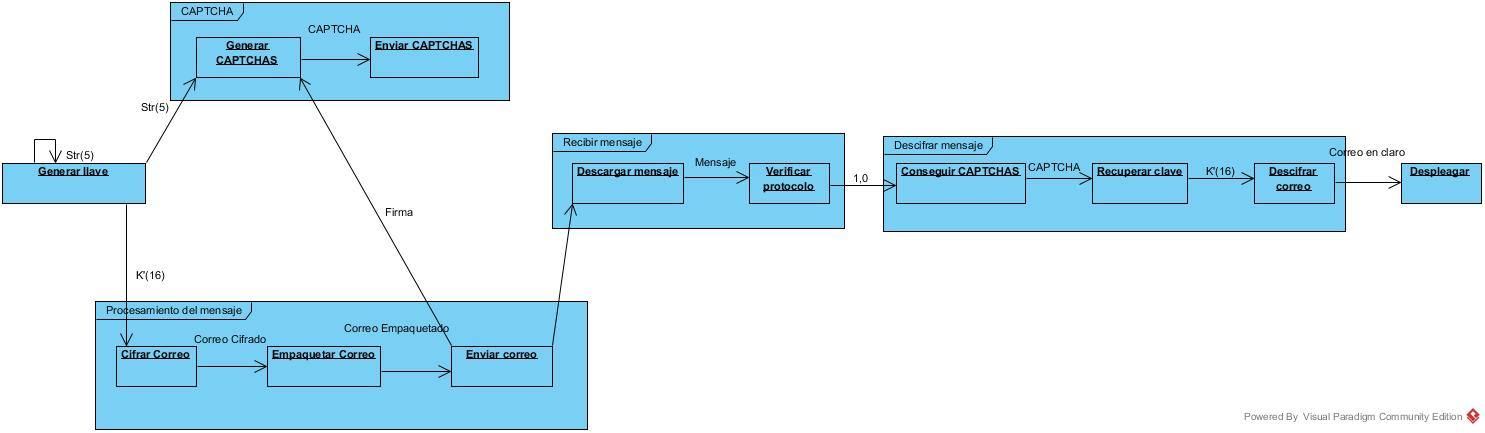
\includegraphics[width=1\linewidth, height=5cm]{./images/bloques0.jpg}
	\caption{Diagrama a bloque 0 general del sistema}
	\label{fig:5-1-1}
\end{figure}
\pagebreak
\begin{table}[H]
 \centering
   {
     \begin{tabular}{| p{2,2cm} | p{1,7cm} | p{2,5cm} | p{3cm} | p{2cm} | p{2,1cm} | p{2cm} |}
     \hline
     & \textbf{Generar clave} & \textbf{Generar CAPTCHA} & \textbf{Procesamiento del mensaje} & \textbf{Recibir mensaje} & \textbf{Descifrar mensaje} & \textbf{Desplegar}\\
     \hline
     \textbf{Entradas} & *Señal de activación & *Cadena de 5 caracteres: Str(5) & *Clave de 16 bytes: K’(16). *Mensaje de correo. & *Correo Cifrado & Verificación (1,0) & *Correo en claro\\
     \hline
     \textbf{Salidas} & *Cadena de 5 caracteres: Str(5) *Clave de 16 bytes: K’(16) & *Señal de envió & *Correo Cifrado & *Verificación (1,0) & *Correo en claro&\\
     \hline
     \textbf{Descripción} & Se activa el proceso generar clave, este crea una palabra de 5 caracteres (Str(5)), procesa la palabra Str(5) por medio de una función hash obteniendo una palabra de 256 caracteres (K(256)) y recorta esta clave a una palabra de 16 caracteres (K’(16)). & Toma la entrada Str(5) y la convierte en una imagen CAPTCHA, Posteriormente inicia una conexión con el servidor de CAPTCHAS para mandarlo a este. & Cifra el mensaje de correo con la clave K’(16), posteriormente lo firma y genera un timbre para saber que fue creado con este esquema y lo empaqueta para su envió. & El cliente hace una petición al servidor y descarga el mensaje de correo electrónico, lo des empaqueta verifica la firma y el timbrado para saber de quién viene y si está cifrado bajo este esquema. & Se hace una petición al servidor de CAPTCHAS, se descargan los CAPTCHAS asociados al correo, ya con el CAPTCHA este se resuelve y se recupera la cadena Str(5), esta se pasa por una función hash y se recupera K(256), esta se corta a K’(16), con esto se descifra el mensaje. & Se muestra el correo descifrado en la interfase del cliente de correo electrónico.\\

    \end{tabular}
    }
    \caption{Diagrama a bloques 0 general}
    \label{tabla:b0}
\end{table}


\newpage
\newpage
%\subsection{Diagrama a bloques 1 Generar clave}
\begin{figure}[H]
	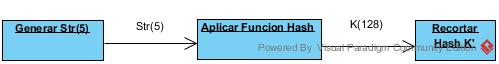
\includegraphics[width=1\linewidth, height=2cm]{./images/bloques1.jpg}
	\caption{Diagrama a bloques 1 Generar clave}
	\label{fig:5-2-1}
\end{figure}
\begin{table}[H]
 \centering
   {
     \begin{tabular}{| p{4cm} | p{4cm} | p{4cm} | p{4cm} |}
     \hline
     & \textbf{Generar Str(5)} & \textbf{Aplicar Función Hash} & \textbf{Recortar Hash K’}\\
     \hline
     \textbf{Entradas} & *Llamada a Función & *Cadena de 5 caracteres: Str(5) & *Digesto K(128)\\
     \hline
     \textbf{Salidas} & *Cadena de 5 caracteres: Str(5) & *Digesto K(128) & *K’(16)\\
     \hline
     \textbf{Descripción} & Toma una función random módulo 67, para formar una palabra con 5 caracteres aleatorios tomados del siguiente conjunto.Anillo67{-.,+*[a-z][A-Z]} & Se pasa la cadena Str(5) por una función hash SHA-1 para obtener un digesto único de esta palabra. & Se copian a otro string lo primeros 16 caracteres del digesto K(128) para formar la clave K’(16)\\

    \end{tabular}
    }
    \caption{Diagrama a bloques 1 general clave}
    \label{tabla:b1}
\end{table}

\begin{table}[H]
 \centering
   {
     \begin{tabular}{| p{3cm} | p{3cm} |}
     \hline
     & \textbf{Cifrar}\\
     \hline
     \textbf{Entradas} & *Clave K’(16) *Mensaje de correo\\
     \hline
     \textbf{Salidas} & *Correo cifrado\\
     \hline
     \textbf{Descripción} & Se cifra el mensaje con un algoritmo de llave simétrica (AES o DES) usando una llave de 16bytes o 128bits.\\

    \end{tabular}
    }
    \caption{Diagrama a bloques 2 Cifrar Correo}
    \label{tabla:b2}
\end{table}

\begin{figure}[H]
	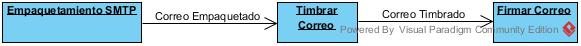
\includegraphics[width=1\linewidth, height=1cm]{./images/bloques3.jpg}
	\caption{Diagrama a bloques 3 Empaquetar Correo}
	\label{fig:5-3-1}
\end{figure}

\begin{table}[H]
 \centering
   {
     \begin{tabular}{| p{4cm} | p{4cm} | p{4cm} |}
     \hline
     & \textbf{Empaquetamiento SMTP} & \textbf{Timbrar Correo}\\
     \hline
     \textbf{Entradas} & *Mensaje Cifrado & *Correo Empaqueta\\
     \hline
     \textbf{Salidas} & *Correo Empaquetado & *Correo Timbrado\\
     \hline
     \textbf{Descripción} & Se toma el correo y se integra en el formato del correo marcado en el RFC822 & Se timbra el mensaje colocando una marca después del final del mensaje. Para señalar que el correo enviado está cifrado bajo este protocolo.\\

    \end{tabular}
    }
    \caption{Diagrama a bloques 3 Empaquetar Correo}
    \label{tabla:b3}
\end{table}

\begin{figure}[H]
	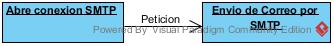
\includegraphics[width=1\linewidth, height=2cm]{./images/bloques4.jpg}
	\caption{Diagrama a bloques 4 Enviar correo}
	\label{fig:5-4-1}
\end{figure}

\begin{table}[H]
 \centering
   {
     \begin{tabular}{| p{4cm} | p{4cm} | p{4cm} |}
     \hline
     & \textbf{Abrir conexión SMTP} & \textbf{Envió de Correo por SMTP}\\
     \hline
     \textbf{Entradas} & *Petición & *Correo empaquetado\\
     \hline
     \textbf{Salidas} & *Canal de comunicación & *Confirmación de envió\\
     \hline
     \textbf{Descripción} & Se genera una petición para conexión SMTP  & Se manda el correo electrónico al servidor por medio del protocolo SMTP\\

    \end{tabular}
    }
    \caption{Diagrama a bloques 4 Enviar correo}
    \label{tabla:b4}
\end{table}
\clearpage
\begin{figure}[H]
	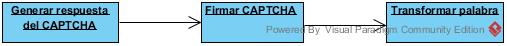
\includegraphics[width=1\linewidth, height=2cm]{./images/bloques5.jpg}
	\caption{Diagrama a bloques 5 Generar CAPTCHA}
	\label{fig:5-5-1}
\end{figure}
\begin{table}[H]
 \centering
   {
     \begin{tabular}{| p{4cm} | p{4cm} | p{4cm} | p{4cm} |}
     \hline
     & \textbf{Generar respuesta del CAPTCHA} & \textbf{Firmar CAPTCHA} & \textbf{Transformar palabra}\\
     \hline
     \textbf{Entradas} & *Cadena de caracteres: Str(5) & *Firma & *Señal de confirmación\\
     \hline
     \textbf{Salidas} & *Señal de confirmación & *Archivo Firmado & *Imagen CAPTCHA\\
     \hline
     \textbf{Descripción} & Genera un archivo con la respuesta del CAPTCHA  & Se firma el CAPTCHA por medio de un Hashing del mensaje. & Convierte el Str(5) en una imagen distorsionada que llamaremos CAPTCHA\\

    \end{tabular}
    }
    \caption{Diagrama a bloques 5 Generar CAPTCHA}
    \label{tabla:b5}
\end{table}
\newpage
\begin{figure}[H]
	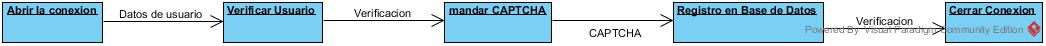
\includegraphics[width=1\linewidth, height=1cm]{./images/bloques6.jpg}
	\caption{Diagrama a bloques 6 Enviar CAPTCHAS (Usuario existente)}
	\label{fig:5-6-1}
\end{figure}

\begin{table}[H]
 \centering
   {
     \begin{tabular}{| p{2,5cm} | p{2,5cm} | p{2,5cm} | p{2,5cm} | p{2,5cm} | p{2,5cm} |}
     \hline
     & \textbf{Abrir conexión} & \textbf{Verificar Usuario} & \textbf{Mandar CAPTCHA} & \textbf{Registrar en base de datos} & \textbf{Cerrar Conexión}\\
     \hline
     \textbf{Entradas} & *CAPTCHAS & *Datos de Usuario & *Verificación de usuario & *Datos de usuario *CAPTCHA & Verificación\\
     \hline
     \textbf{Salidas} & *Datos de usuario & *Verificación de usuario & *CAPTCHA & Verificación &\\
     \hline
     \textbf{Descripción} & Se genera una petición para poder entablar una conexión con el servidor de CAPTCHAS & Se verifica la existencia del usuario en el servidor, si existe se le da acceso & Ya verificado el usuario se manda el CAPTCHA al servidor & Se registran los datos del CAPTCHA en la base de datos y se envía una verificación & Se cierra la conexión y se guardan los datos\\

    \end{tabular}
    }
    \caption{Diagrama a bloques 6 Enviar CAPTCHAS (Usuario existente)}
    \label{tabla:b6}
\end{table}
\pagebreak
\begin{figure}[H]
	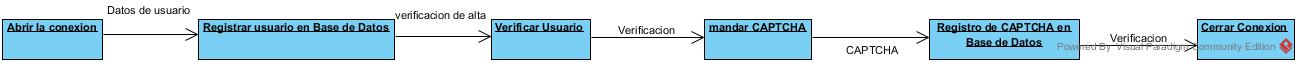
\includegraphics[width=1\linewidth, height=1cm]{./images/bloques7.jpg}
	\caption{Diagrama a bloques 7 Enviar CAPTCHAS (Usuario inexistente)}
	\label{fig:5-7-1}
\end{figure}
\begin{table}[H]
 \centering
   {
     \begin{tabular}{| p{2cm} | p{2cm} | p{2,5cm} | p{2cm} | p{2,5cm} | p{2,5cm} | p{2cm} |}
     \hline
     & \textbf{Abrir conexión} & \textbf{Registrar usuario en Base de Datos} & \textbf{Verificar Usuario} & \textbf{Mandar CAPTCHA} & \textbf{Registrar en base de datos} & \textbf{Cerrar Conexión}\\
     \hline
     \textbf{Entradas} & *CAPTCHAS & *Datos de Usuario & *Verificación de registro & *Verificación de usuario & *Datos de usuario *CAPTCHA & Verificación\\
     \hline
     \textbf{Salidas} & *Datos de usuario & *Verificación de registro & *Verificación de usuario & *CAPTCHA & Verificación &\\
     \hline
     \textbf{Descripción} & Se genera una petición para poder entablar una conexión con el servidor de CAPTCHAS & Se da de alta al usuario en la base de datos & se le da acceso  al usuario & Ya verificado el usuario se manda el CAPTCHA al servidor & Se registran los datos del CAPTCHA en la base de datos y se envía una verificación & Se cierra la conexión y se guardan los datos\\

    \end{tabular}
    }
    \caption{Diagrama a bloques 7 Enviar CAPTCHAS (Usuario inexistente)}
    \label{tabla:b7}
\end{table}
\pagebreak
\begin{figure}[H]
	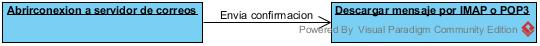
\includegraphics[width=1\linewidth, height=1cm]{./images/bloques8.jpg}
	\caption{Diagrama a bloques 8 Descargar mensaje}
	\label{fig:5-8-1}
\end{figure}
\begin{table}[H]
 \centering
   {
     \begin{tabular}{| p{3cm} | p{4cm} | p{4cm} |}
     \hline
     & \textbf{Abrir conexión al servidor de correo} & \textbf{Descargar mensaje por IMAP o POP3}\\
     \hline
     \textbf{Entradas} & *Señal de activación & *Confirmación\\
     \hline
     \textbf{Salidas} & *Confirmación & *Correo electrónico\\
     \hline
     \textbf{Descripción} & El receptor se conecta al servidor de correo electrónico e inicia la sesión & Descarga del servidor de correo electrónico todos los mensajes que aún no se hayan descargado.\\

    \end{tabular}
    }
    \caption{Diagrama a bloques 8 Descargar mensaje}
    \label{tabla:b8}
\end{table}
\begin{figure}[H]
	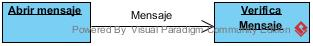
\includegraphics[width=1\linewidth, height=1cm]{./images/bloques9.jpg}
	\caption{Diagrama a bloques 9 Verificar protocolo (con protocolo válido)}
	\label{fig:5-9-1}
\end{figure}
\begin{table}[H]
 \centering
   {
     \begin{tabular}{| p{3cm} | p{4cm} | p{4cm} |}
     \hline
     & \textbf{Abrir mensaje} & \textbf{Verificar mensaje}\\
     \hline
     \textbf{Entradas} & *Correo electrónico & *mensaje\\
     \hline
     \textbf{Salidas} & *Mensaje & *verificación\\
     \hline
     \textbf{Descripción} & Se toma el mensaje descargado del servidor y se des empaqueta para dejar solo el texto del mensaje & Se verifica que el mensaje tenga la bandera correspondiente a que está cifrado con este esquema\\

    \end{tabular}
    }
    \caption{Diagrama a bloques 9 Verificar protocolo (con protocolo válido)}
    \label{tabla:b9}
\end{table}


\clearpage
\begin{table}[H]
 \centering
   {
     \begin{tabular}{| p{3cm} | p{4cm} | p{4cm} |}
     \hline
     & \textbf{Abrir mensaje} & \textbf{Verificar mensaje}\\
     \hline
     \textbf{Entradas} & *Correo electrónico & *mensaje\\
     \hline
     \textbf{Salidas} & *Mensaje & *verificación\\
     \hline
     \textbf{Descripción} & Se toma el mensaje descargado del servidor y se des empaqueta para dejar solo el texto del mensaje & Si la verificación es negativa se manda directamente al bloque de Despliegue\\

    \end{tabular}
    }
    \caption{Diagrama a bloques 10 Verificar protocolo (con protocolo inválido)	}
    \label{tabla:b10}
\end{table}

\begin{figure}[H]
	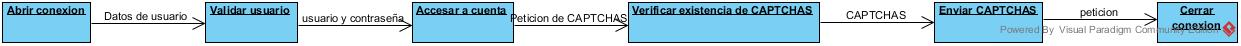
\includegraphics[width=1\linewidth, height=1cm]{./images/bloques11.jpg}
	\caption{Diagrama a bloques 11 Conseguir CAPTCHAS (Usuario existente)}
	\label{fig:5-11-1}
\end{figure}
\begin{table}[H]
 \centering
   {
     \begin{tabular}{| p{2,5cm} | p{3cm} | p{2cm} | p{2cm} | p{3cm} | p{3cm} |}
     \hline
     & \textbf{Abrir Conexión} & \textbf{Validar Usuario} & \textbf{Accesar a cuenta} & \textbf{Verificar existencia de CAPTCHA} & \textbf{Enviar CAPTCHA}\\
     \hline
     \textbf{Entradas} & *Confirmación & *Datos usuario & *Contraseña & *Petición de CAPTCHAS & *Confirmación\\
     \hline
     \textbf{Salidas} & *verificación & *Contraseña & *confirmación & *confirmación & *CAPTCHA\\
     \hline
     \textbf{Descripción} & Se abre una conexión con el servidor de CAPTCHAS & Se verifica que el usuario este dado de alta en el servidor mandándole una petición a la base de datos, si el usuario existe se accesa & Si esta dado de alta en el servidor se manda la contraseña para que pueda tener acceso a los CAPTCHAS de su cuenta & Se verifica que los CAPTCHAS que están ligados al mensaje que realizo la petición existan & Si existen estos CAPTCHAS son enviados de regreso al mensaje\\

    \end{tabular}
    }
    \caption{Diagrama a bloques 11 Conseguir CAPTCHAS (Usuario existente)}
    \label{tabla:b11}
\end{table}

\begin{figure}[H]
	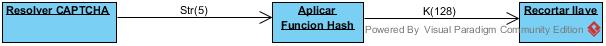
\includegraphics[width=1\linewidth, height=1cm]{./images/bloques12.jpg}
	\caption{Diagrama a bloques 12 Recuperar clave}
	\label{fig:5-12-1}
\end{figure}
\begin{table}[H]
 \centering
   {
     \begin{tabular}{| p{2,5cm} | p{3cm} | p{3cm} | p{3cm} |}
     \hline
     & \textbf{Resolver CAPTCHA} & \textbf{Aplicar Función Hash} & \textbf{Recortar llave}\\
     \hline
     \textbf{Entradas} & *CAPTCHA & *Cadena de 5 caracteres: Str(5) & *Digesto K(128)\\
     \hline
     \textbf{Salidas} & *Str(5) & *Digesto K(128) & *K’(16)\\
     \hline
     \textbf{Descripción} & Se despliega el CAPTCHA para que el usuario pueda resolverlo & Se pasa la cadena Str(5) por una función hash SHA-1 para obtener un digesto único de esta palabra & Se copian a otro string lo primeros 16 caracteres del digesto K(128) para formar la clave K’(16)\\

    \end{tabular}
    }
    \caption{Diagrama a bloques 12 Recuperar clave}
    \label{tabla:b12}
\end{table}
\begin{table}[H]
 \centering
   {
     \begin{tabular}{| p{2,5cm} | p{3cm} |}
     \hline
     & \textbf{Descifrar}\\
     \hline
     \textbf{Entradas} & *Clave K’(16) *Mensaje de correo\\
     \hline
     \textbf{Salidas} & *Correo descifrado\\
     \hline
     \textbf{Descripción} & Se descifra el mensaje con un algoritmo de llave simétrica (AES o DES) usando una llave de 16bytes o 128bits.\\

    \end{tabular}
    }
    \caption{Diagrama a bloques 13 Descifrar correo}
    \label{tabla:b13}
\end{table}

